\documentclass{article}
\usepackage{MNotes}
\usepackage{amssymb}
\usepackage{bussproofs}
\title{\huge{\textbf{Assignment 3}}}
\author{\Chi{杨乐天}}
\date{}

\newcommand \ran[1]							{\text{Ran}\left( #1 \right)}
\newcommand \logequiv						{\vDash\mathrel{\text{\reflectbox{$\vDash$}}}}

\begin{document}
\maketitle

\section*{Problem 1}

Suppose (a) holds but (b) doesn't. Then there exists a finitely satisfiable $\Gamma$ that is not satisfiable.

Notice that $\Sigma \vDash \alpha$ is equivalent to $\Sigma; \neg\alpha$ is unsatisfiable. Then the corollary is exactly saying that if $\Sigma; \beta$ is unsatisfiable, then there exists finite $\Delta \subseteq \Sigma$ such that $\Delta; \beta$ is unsatisfiable, where $\beta$ is any wff.

Since $\Gamma$ is unsatisfiable, then we let $\Gamma = \Gamma' \cup \{ \beta \}$ such that $\Gamma' \cap \{ \beta \} = \varnothing$. Then we know from the corollary that there exists finite $\Delta' \subseteq \Gamma'$ such that $\Delta'; \beta$ is unsatisfiable. However, $\Delta'; \beta$ is a finite subset of $\Gamma$, which contradicts with the assumption that $\Gamma$ is finitely satisfiable.



\section*{Problem 2}

\begin{figure}[htbp]
	\centering
	\subfloat{\includegraphics[width=0.4\linewidth]{tree1.jpg}}
	\hfill
	\subfloat{\includegraphics[width=0.4\linewidth]{tree2.jpg}}
	\hfill
	\\
	\subfloat{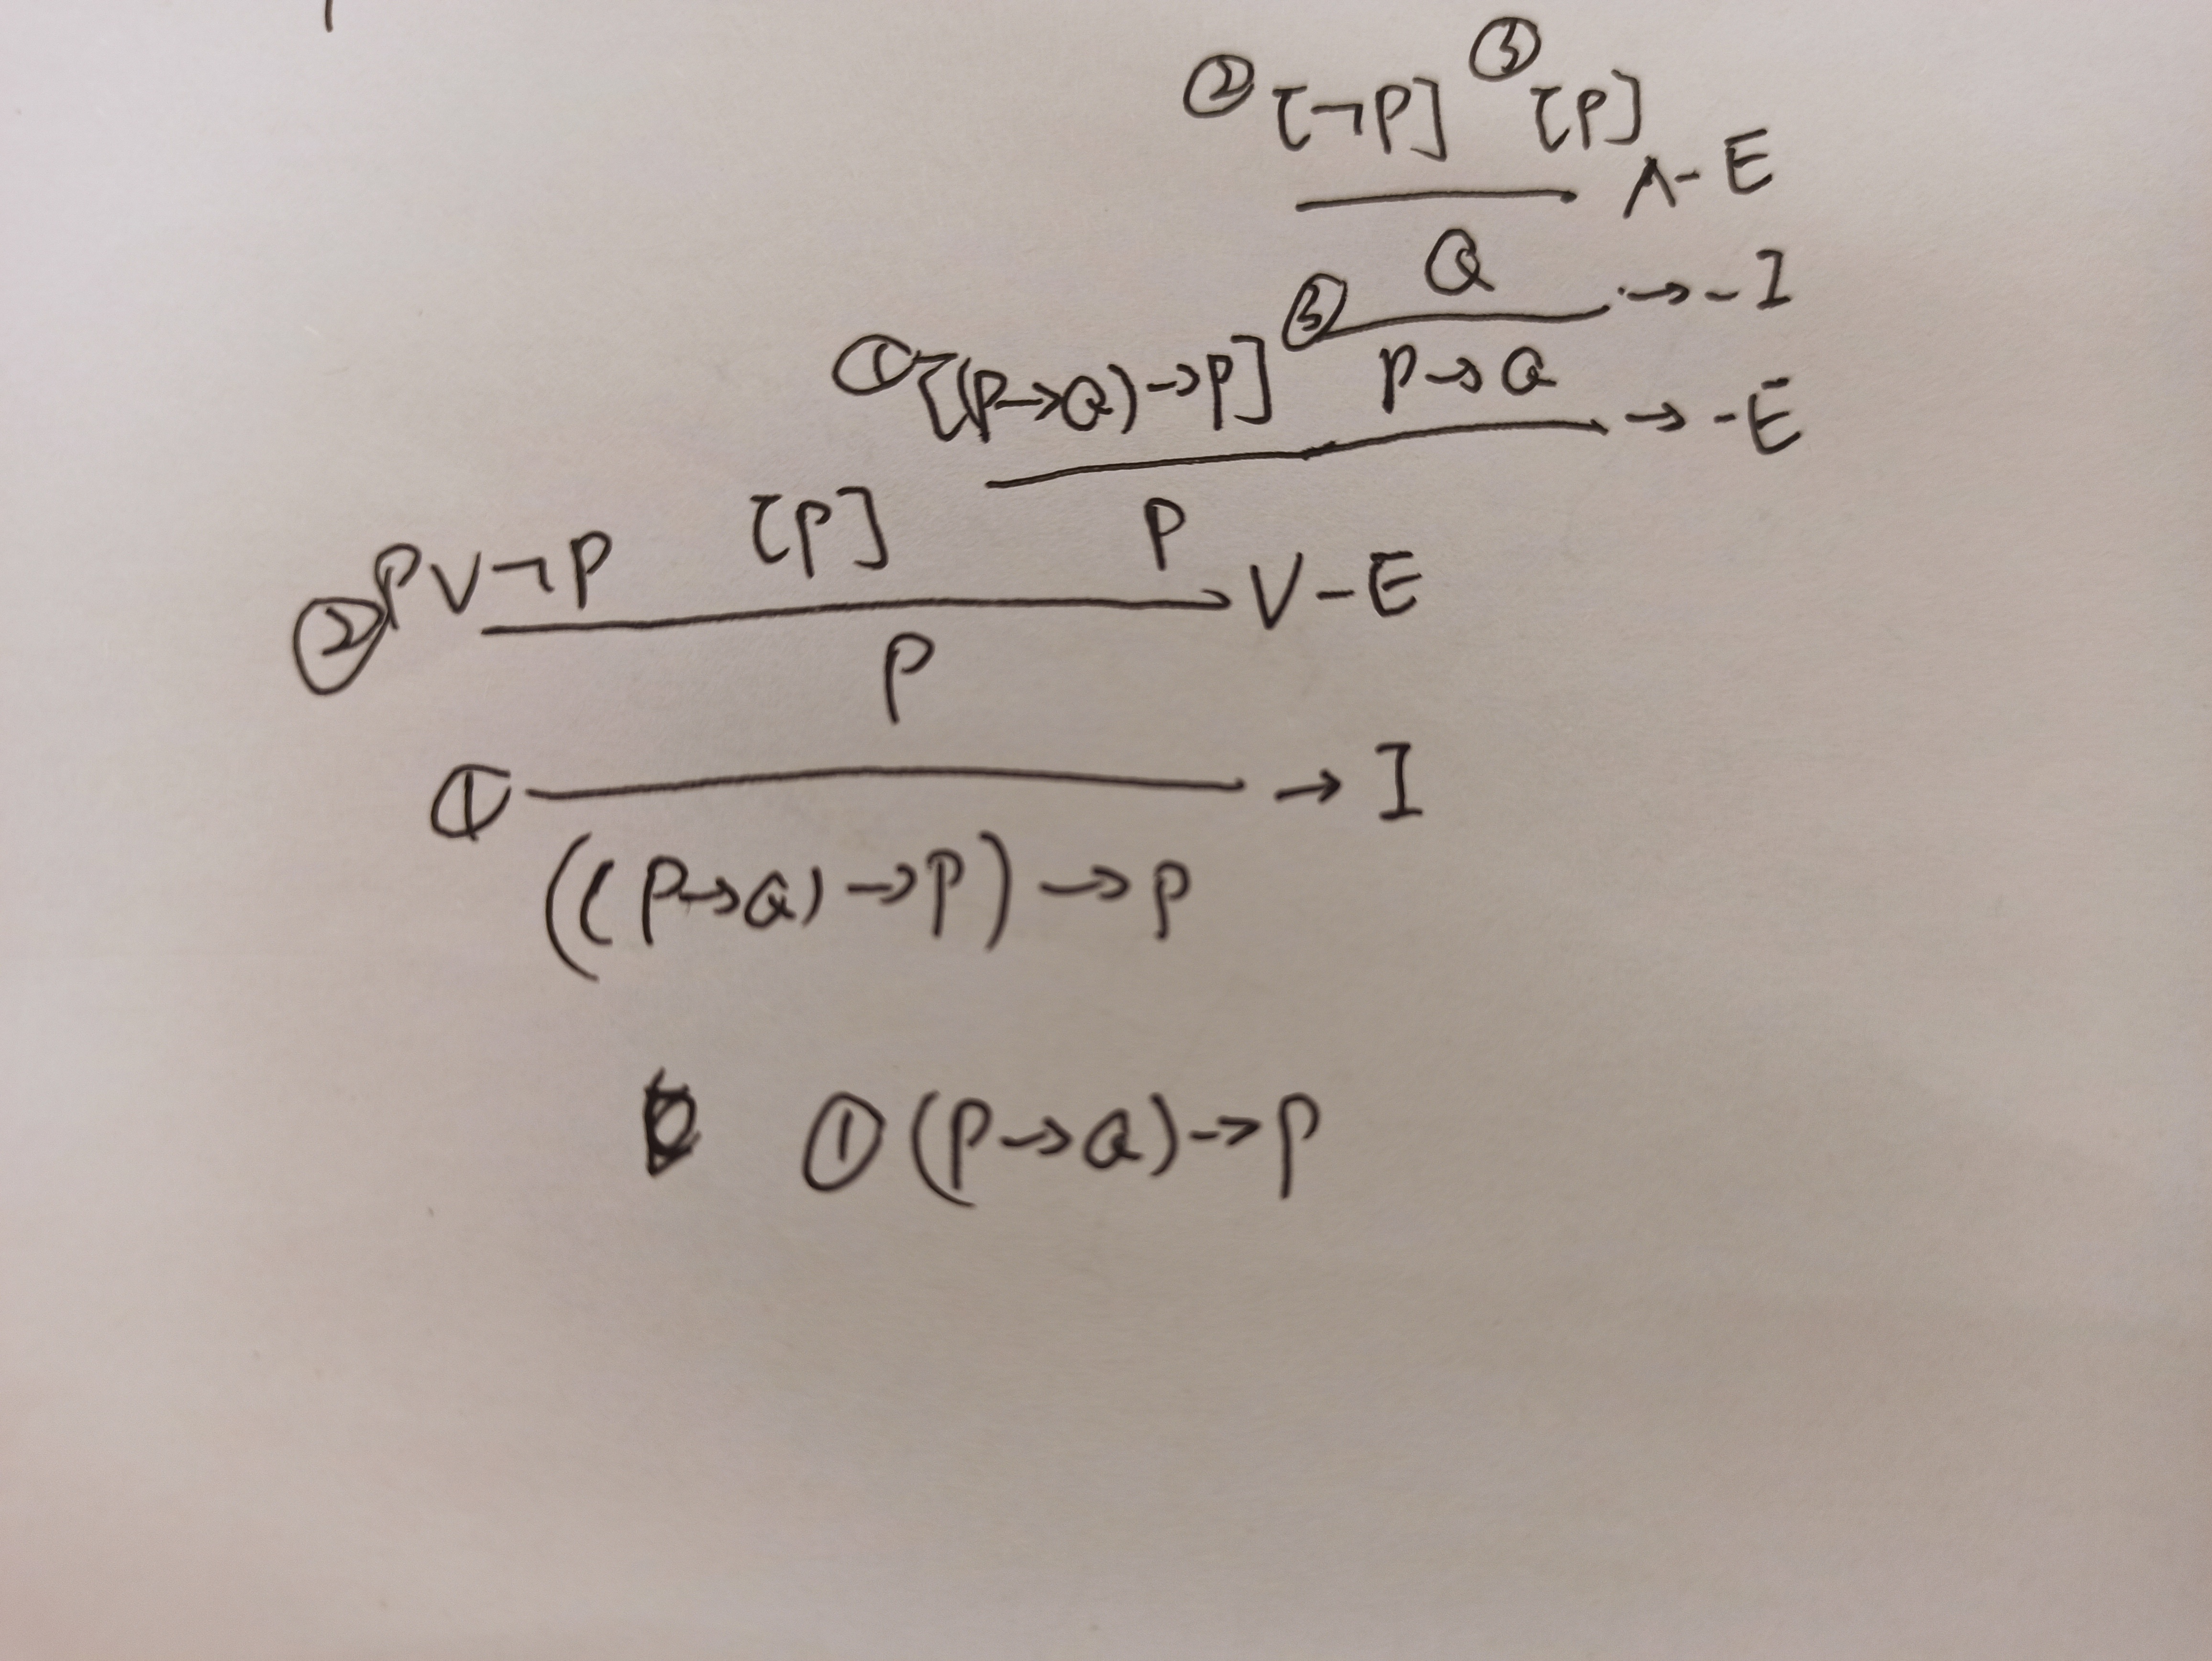
\includegraphics[width=0.4\linewidth]{tree3.jpg}}
\end{figure}

\section*{Problem 3}

\subsection*{3.a}

We already have partial proof tree $\displaystyle \frac{\sigma_1 \sigma_2 ... \sigma_n}{\alpha}$ where $\{\sigma_1,\sigma_2,...,\sigma_n\} \subseteq \Sigma$ and $\displaystyle \frac{\alpha \delta_1 ... \delta_m}{\beta}$ where $\{\delta_1,...,\delta_m\} \subseteq \Delta$.

Then we can construct new tree $\displaystyle \frac{\displaystyle \frac{\sigma_1 \sigma_2 ... \sigma_n}{\alpha} \delta_1 ... \delta_m}{\beta}$ as a partial proof tree of $\Sigma \cup \Delta \vdash \beta$.

\subsection*{3.b}

We have
\begin{prooftree}
\AxiomC{$\gamma_1$} \AxiomC{$\gamma_2$} \AxiomC{$...$} \AxiomC{$\gamma_n$} \AxiomC{$\alpha$}
\doubleLine
\QuinaryInfC{$\beta \leftrightarrow \neg\beta$}
\end{prooftree}
where $\{\gamma_1,\gamma_2,...,\gamma_n\} \subseteq \Gamma$.

Then we build several partial proof trees.

\begin{prooftree}
		\AxiomC{$\beta$}
			\AxiomC{$\gamma_1$} \AxiomC{$\gamma_2$} \AxiomC{$...$} \AxiomC{$\gamma_n$} \AxiomC{$\alpha$}
			\doubleLine
			\QuinaryInfC{$\beta \leftrightarrow \neg\beta$}
		\RightLabel{$\leftrightarrow\text{-E}_1$}
		\UnaryInfC{$\beta \to \neg\beta$}
	\RightLabel{$\to$-E}
	\BinaryInfC{$\neg\beta$}
	\AxiomC{$\beta$}
\RightLabel{$\land$-I}
\BinaryInfC{$\beta \land \neg\beta$}
\end{prooftree}

Substituting $\beta$ and $\neg\beta$ with each other, we can build a symmetric partial proof tree of $\Gamma \cup \{ \alpha, \neg\beta \} \vdash \beta \land \neg\beta$.

\begin{prooftree}
	\AxiomC{$\alpha \lor \neg\alpha$}
			\AxiomC{$\beta \lor \neg\beta$}
				\AxiomC{$\Gamma; [\alpha], [\beta]$}
			\doubleLine
			\UnaryInfC{$\beta \land \neg\beta$}
				\AxiomC{$\Gamma; [\alpha], [\neg\beta]$}
			\doubleLine
			\UnaryInfC{$\beta \land \neg\beta$}
		\RightLabel{$\lor\text{-E}$}
		\TrinaryInfC{$\beta \land \neg\beta$}
	\RightLabel{$\land\text{-E}$}
	\UnaryInfC{$\neg\alpha$}
	\AxiomC{$[\neg\alpha]$}
\RightLabel{$\lor\text{-E}$}
\TrinaryInfC{$\neg\alpha$}
\end{prooftree}

Then we have shown that $\Sigma \vdash \neg\alpha$.

\section*{Problem 4}

\subsection*{4.a}

From the proof tree we know that the conclusion is dependent only on the assumption $\alpha \lor \neg\alpha$.
\begin{figure}[htbp]
	\centering
	\includegraphics[width=7cm]{tree4.jpg}
\end{figure}

\subsection*{4.b}

From the proof tree we know that the conclusion is dependent only on the assumption $(\alpha \to \beta) \to (\neg\alpha \lor \beta)$.
\begin{figure}[htbp]
	\centering
	\includegraphics[width=7cm]{tree5.jpg}
\end{figure}


\section*{Problem 5}

\subsection*{5.a}

\begin{align*}
	&(\neg A \lor \neg B) \to \neg ( A \land B )
	\\
	\Leftrightarrow &
	((A \to \perp) \lor (B \to \perp)) \to ((A \land B) \to \perp)
\end{align*}

\subsection*{5.b}

\begin{figure}[htbp]
	\centering
	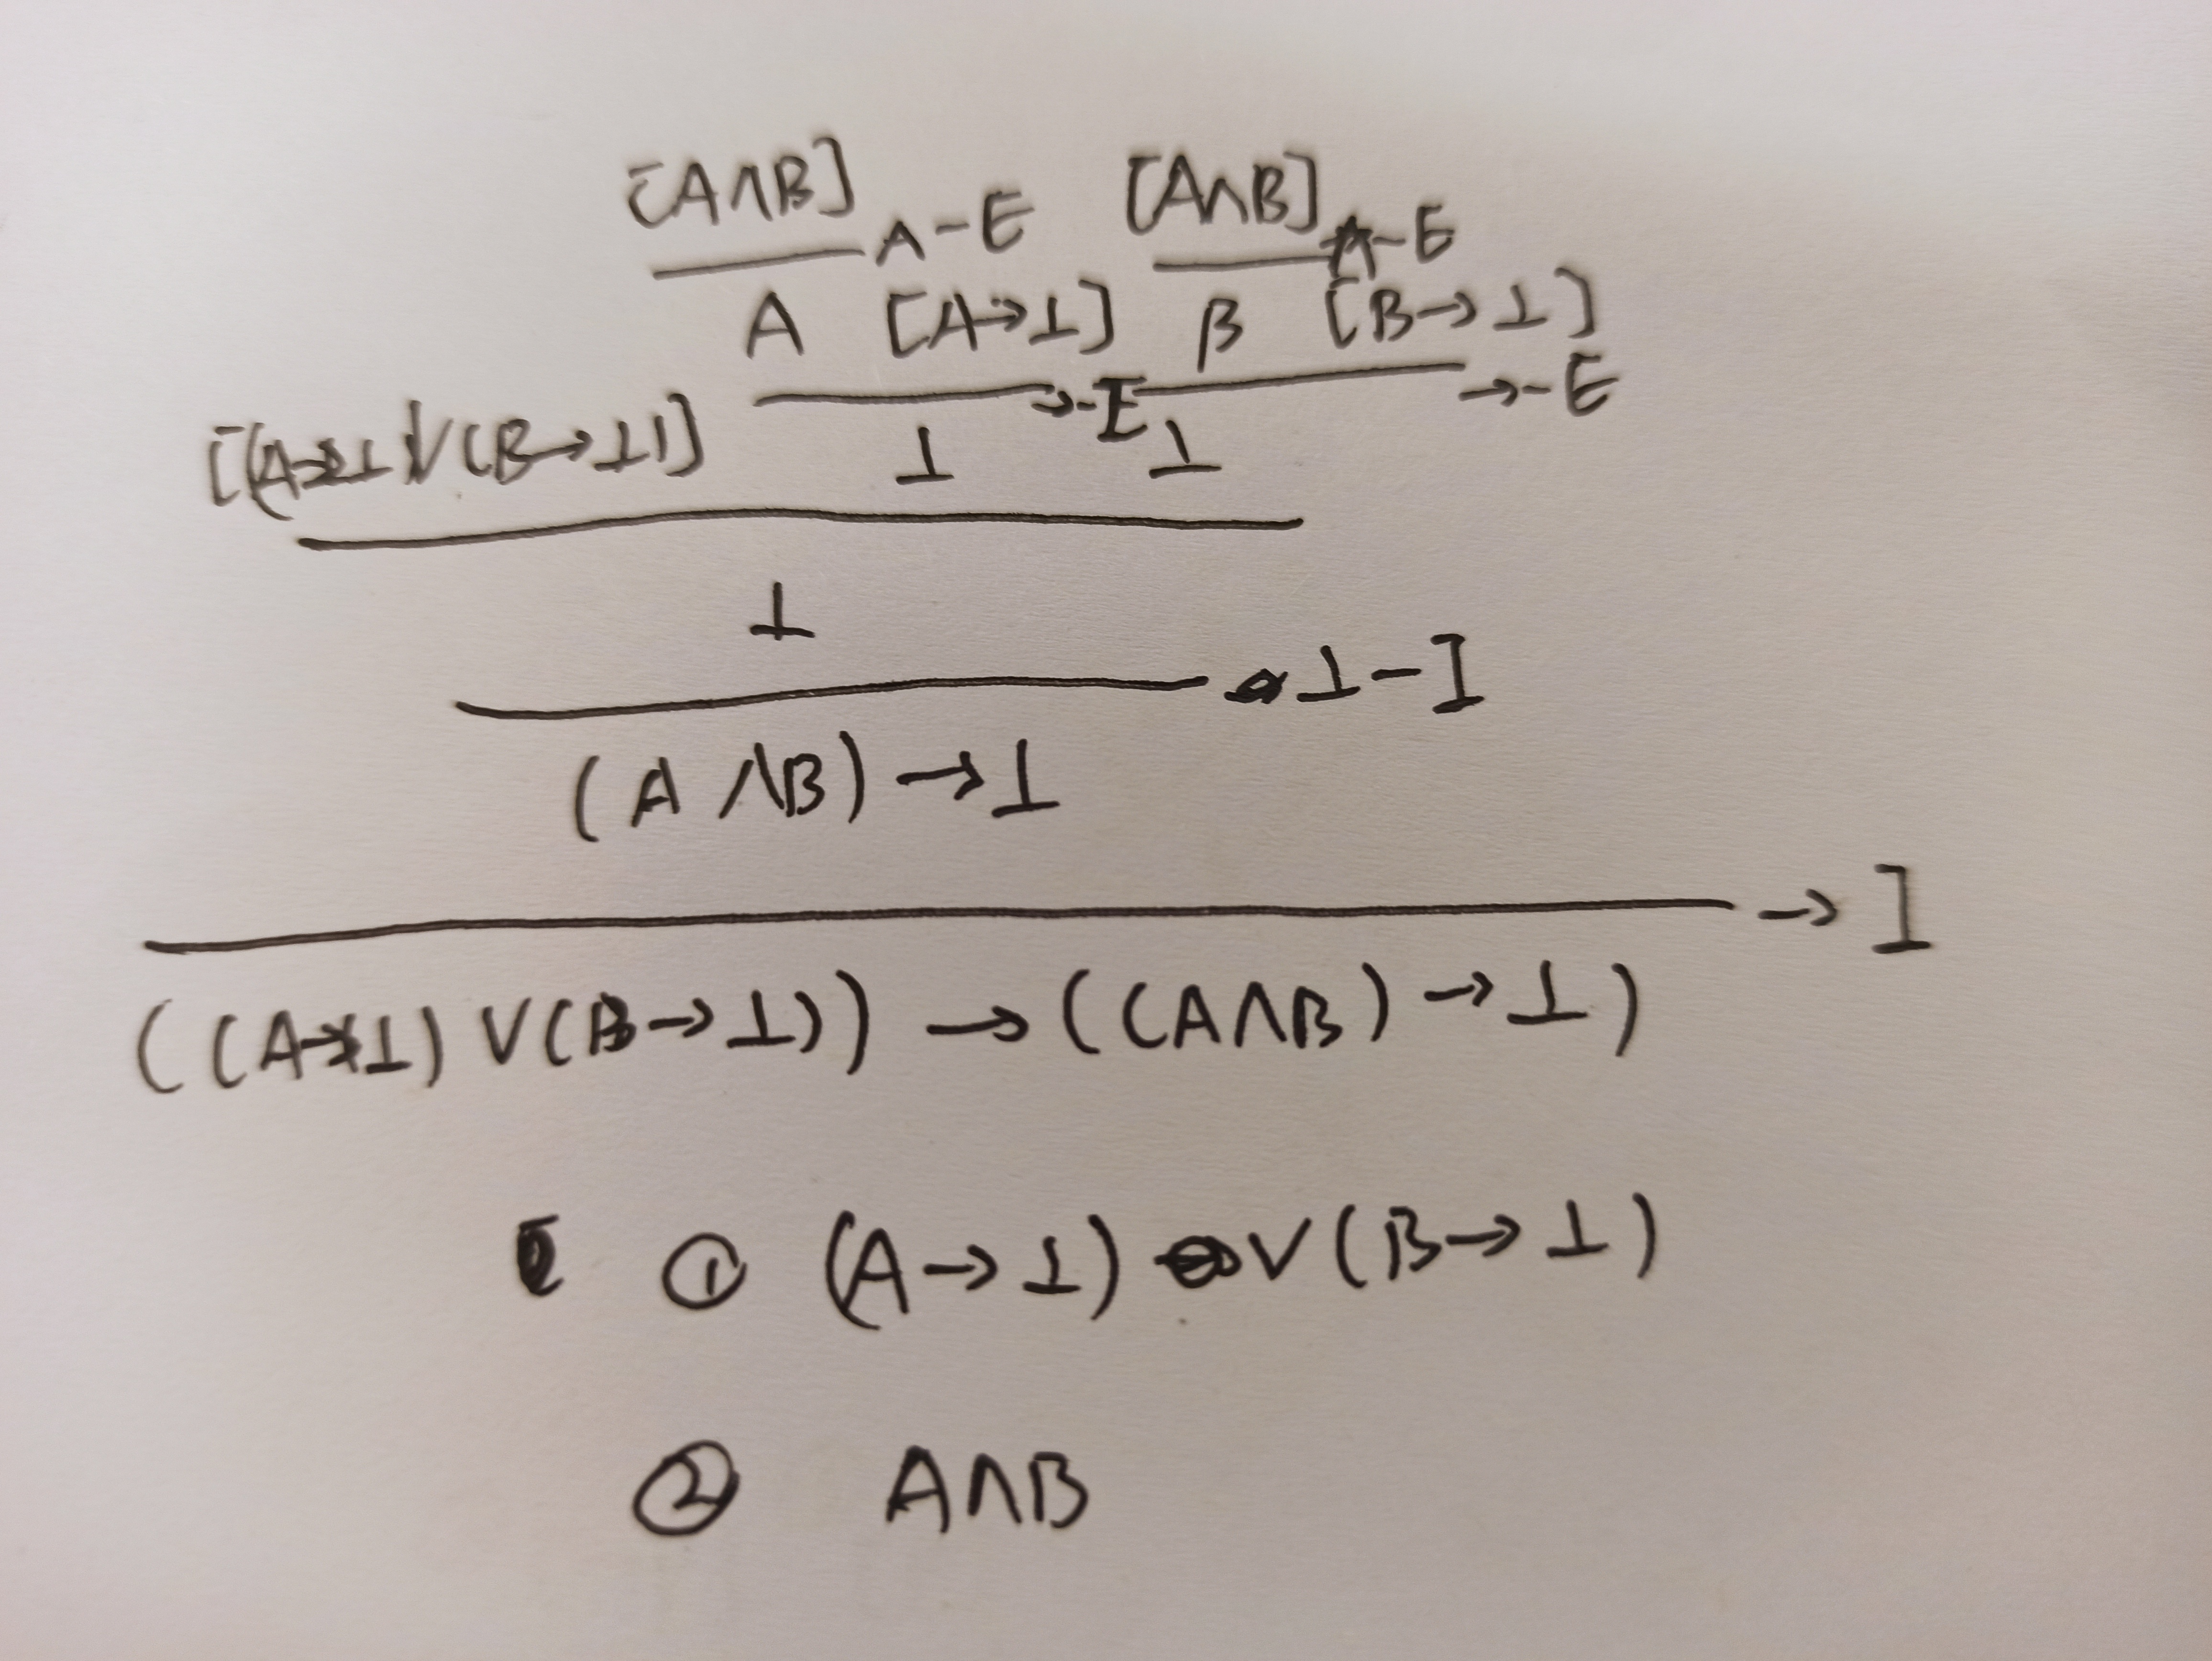
\includegraphics[width=7cm]{tree6.jpg}
\end{figure}



\end{document}